\documentclass[border=4pt]{standalone}
% Preámbulo común de las figuras. Cada figura es un documento standalone
% que se compila a SVG con scripts/build_figures.sh
\usepackage[utf8]{inputenc}
\usepackage{amsmath}
\usepackage{tikz}
\usepackage[american, siunitx]{circuitikz}
\usetikzlibrary{arrows.meta,calc,decorations.pathmorphing,patterns}
\tikzset{
  >={Stealth[length=2.2mm]},
  eje/.style={->, thin},
  hilo/.style={thick},
}
% Paleta común: tonos medios legibles sobre fondo claro
\definecolor{azul}{RGB}{31,94,168}
\definecolor{rojo}{RGB}{192,57,43}
\definecolor{verde}{RGB}{39,128,73}
\definecolor{naranja}{RGB}{211,120,30}
\definecolor{morado}{RGB}{125,60,152}

\begin{document}
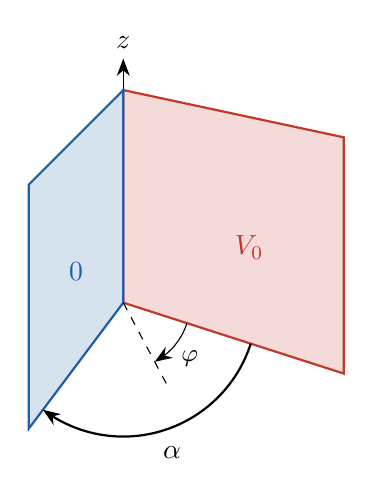
\begin{tikzpicture}[scale=1.0]
  \draw[eje] (0,0.3) -- (0,3.4) node[above]{$z$};
  \filldraw[draw=rojo, fill=rojo!18, thick] (0,0.3) -- (2.8,-0.6) -- (2.8,2.4) -- (0,3.0) -- cycle;
  \filldraw[draw=azul, fill=azul!18, thick] (0,0.3) -- (-1.2,-1.3) -- (-1.2,1.8) -- (0,3.0) -- cycle;
  \node[rojo] at (1.6,1.0) {$V_0$};
  \node[azul] at (-0.6,0.7) {$0$};
  \draw[->, thick] (1.619,-0.220) arc[start angle=-17.8, end angle=-126.9, radius=1.7];
  \node at (0.618,-1.602) {$\alpha$};
  \draw[dashed] (0,0.3) -- (0.587,-0.804);
  \draw[->] (0.809,0.040) arc[start angle=-17.8, end angle=-62.0, radius=0.85];
  \node[font=\small] at (0.844,-0.406) {$\varphi$};
\end{tikzpicture}
\end{document}
